\documentclass[11pt]{article}
\usepackage[scaled=0.92]{helvet}
\usepackage{geometry}
\geometry{letterpaper,tmargin=1in,bmargin=1in,lmargin=1in,rmargin=1in}
\usepackage[parfill]{parskip} % Activate to begin paragraphs with an empty line rather than an indent %\usepackage{graphicx}
\usepackage{amsmath,amssymb, mathrsfs,  mathtools, dsfont}
\usepackage{tabularx}
\usepackage{tikz-cd}
\usepackage[font=footnotesize,labelfont=bf]{caption}
\usepackage{graphicx}
\usepackage{xcolor}
%\usepackage[linkbordercolor ={1 1 1} ]{hyperref}
%\usepackage[sf]{titlesec}
\usepackage{natbib}
%\usepackage{tikz-cd}

\usepackage{../../Tianpei_Report}

%\usepackage{appendix}
%\usepackage{algorithm}
%\usepackage{algorithmic}

%\renewcommand{\algorithmicrequire}{\textbf{Input:}}
%\renewcommand{\algorithmicensure}{\textbf{Output:}}



\begin{document}
\title{Lecture 3:  Theoretical Analysis of Boosting Methods}
\author{ Tianpei Xie}
\date{Feb. 6th., 2023}
\maketitle
\tableofcontents
\newpage
\section{Boosting Algorithm}
\subsection{AdaBoost}
\begin{figure}
\begin{minipage}[t]{1\linewidth}
  \centering
  \centerline{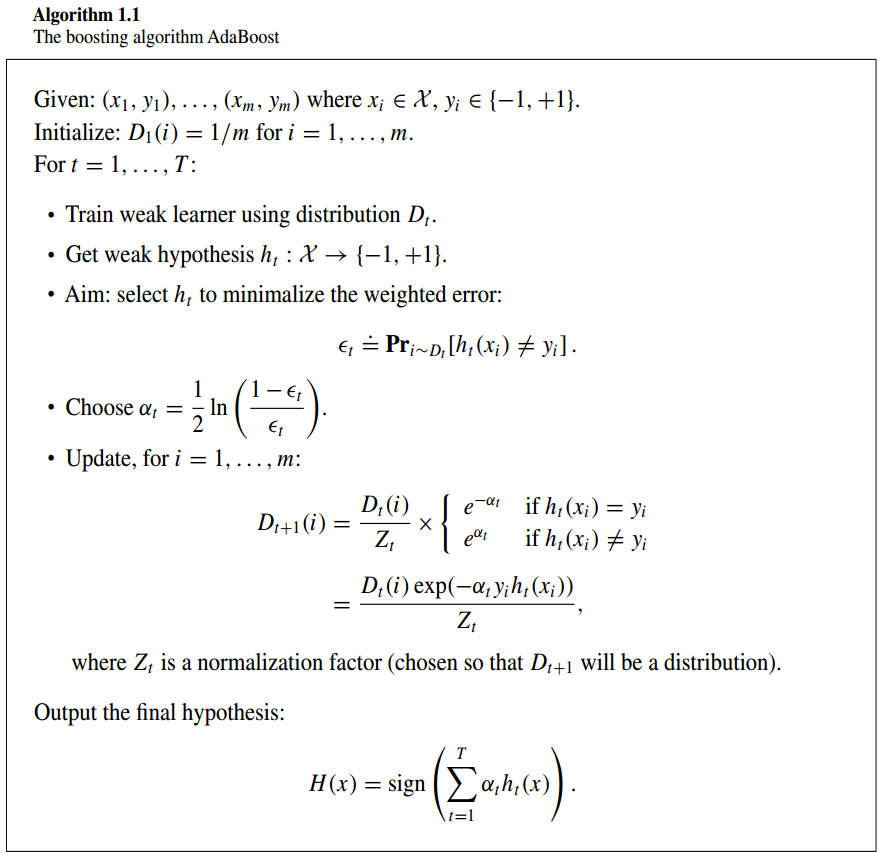
\includegraphics[scale = 0.4]{adaboost.png}}
\end{minipage}
\caption{\footnotesize{\textbf{AdaBoost Algorithm \citep{schapire2012boosting}}}}
\label{fig: adaboost}
\end{figure}

\begin{itemize}
\item \emph{\textbf{The AdaBoost algorithm}} is the first boosting algorithms proposed by Freund and Schapire \citep{schapire2012boosting}. Its basic idea is to combine multiple \emph{weak learners} to form a \emph{strong learner}. This strategy is called \emph{\textbf{ensemble learning}}. Let $h_t \in \cH$ be base hypothesis, and $\alpha_t$ be the corresponding weight at iteration $t \in [1,T]$. The \emph{combined learner} after $T$ iteration is
\begin{align*}
H(x) := \sgn{\sum_{t=1}^{T}\alpha_t h_t(x)}
\end{align*}

\item \begin{remark}
There are several other \emph{ensemble learning algorithms} such that \emph{\textbf{bagging algorithms}}, which is based on \emph{\textbf{boostrap resampling stretegy}}. The idea is to \emph{sample with replacement} on the existing dataset to create \emph{duplicated records}. The most frequent seen records in the existing data are more likely be sampled thus this idea is equivalent to \emph{\textbf{Monte Carlo sampling}} according to the empirical distribution. For each resampled dataset, we can train a classifier that reflect our understanding on the duplicated sample. Then we combine multiple classifier to build a single classifier via \emph{\textbf{decision fusion}}. The typical bagging-based algorithm is \emph{\textbf{the random forest algorithm}}, which build decision trees for each boostrapped dataset and combine them.
\end{remark}

\item \begin{remark}(\textbf{\emph{Characteristic of AdaBoost}}) \\
\emph{AdaBoost} is an \emph{ensemble learning method}. The followings are several key characteristics:
\begin{enumerate}
\item  \emph{\textbf{AdaBoost}}  trains \emph{\textbf{multiple weak learners}} in \underline{\emph{\textbf{sequential manner}}}. Unlike \emph{bagging methods}, \emph{boosting methods} build weak learners \emph{sequentially}. \emph{\textbf{The performance of the previous learners} will \textbf{affect} \textbf{how the new weak-learner is trained}}. In the case of AdaBoost, it will be reflected in \emph{the sample weights}, with misclassified samples having increased weight. 

In this way, it is described as a \underline{\emph{\textbf{functional gradient descent algorithm}}} which \emph{instead of computing the gradient}, it \emph{learns \textbf{a new base hypothesis} that \textbf{resembles} \textbf{the gradient of functional}}.


\item \emph{\textbf{The performance measure}} in each step of \emph{\textbf{AdaBoost}} is \emph{\textbf{the training error rate}} of new base learner relative to \emph{\textbf{a weighted sample distribution}}; i.e.
\begin{align*}
\epsilon_t := \Em{\cD_t}{h_t(X) \neq Y} = \sum_{i=1}^{m}\cD_t(i) \ind{h_t(X_i)}
\end{align*} The training error rate under $\cD_t$ has two roles:
\begin{enumerate}
\item it deterime \emph{the \textbf{weight} $\alpha_t$ for the base hypothesis $h_t$.} In AdaBoost, 
\begin{align*}
\alpha_t = \frac{1}{2}\log\paren{\frac{1 - \epsilon_t}{\epsilon_t}}.
\end{align*} It is clear that when the classifier $h_t$ is no more than a random guess with $\epsilon_t = 1/2$, the corresponding weight $\alpha_t = 0$. In other situation, the \emph{smaller} the $\epsilon_t$ the \emph{larger} the $\alpha_t$. Note that $\alpha_t >0$ \emph{\textbf{if and only if}} $\epsilon_t < 1/2$ meaning that the learned hypothesis $h_t$ is a \emph{weak-learner}.

\item it determines \emph{\textbf{the multiplicative factor} in the exponential reweight strategy for each sample}. In particular, the factor is $\exp\paren{-\alpha_t y_i h_t(x_i)}$.
\end{enumerate}

\item \emph{\textbf{AdaBoost} apply an \textbf{\underline{exponential reweighting strategy}} at each iteration}. In particular, 
\begin{align*}
\cD_{t+1}(i) &= \frac{\cD_t}{Z_t} \times \left\{\begin{array}{cc}
e^{-\alpha_t} &\text{if }h_t(x_i) = y_i \\
e^{\alpha_t} &\text{if }h_t(x_i) \neq y_i 
\end{array}
\right.
\end{align*} where $Z_t := \sum_{i=1}^{m}\cD_t(i)\exp\paren{-\alpha_t y_i h_t(x_i)}$ is the partition function that normalized the sample distribution $\cD_{t+1}$. The exponential reweighting strategy \emph{\textbf{shrinks}} the weight by $e^{-\alpha_t} < 1$ when \emph{the sample is correctly labeled}, while \emph{\textbf{enlarges}} the weight by $e^{\alpha_t} > 1$ when \emph{the sample is \textbf{incorrectly labeled}}. This means that \emph{misclassified samples will have \textbf{higher weights}} in next iteration.

\item \emph{AdaBoost} promote the idea of \underline{\emph{\textbf{adversarial learning}}} that is shown great success in deep learning models such as \emph{Generative Adversarial Network (GAN)}. The key idea comes from the \underline{\emph{\textbf{two player zero-sum game}}}. Unlike GAN, AdaBoost did not continually re-train the same hypothesis but instead move on to build a new hypothesis for a few misclassified samples.

The change of sample distribution $\cD_t \to \cD_{t+1}$ helps the AdaBoost to \emph{\textbf{boost the impact} of} \underline{\emph{\textbf{adversarial samples}}} for the \emph{new} learner so that it will \emph{\textbf{overemphasize on the past mistakes}}. The consequence is that \emph{\textbf{the later learned} base hypothesis} is \emph{\textbf{more specialized} on a few \textbf{difficult samples}} while \emph{\textbf{the early learned} base hypothesis} is \emph{more generalized for a majority of easy samples}.

In the end, when \emph{the error rate} of new classifier \emph{decreased}, the corresponding \emph{hypothesis weight} $\alpha_t$ will \emph{decrease} and the multiplicative factor will \emph{tends to} $1$, which leades to the sample distribution \emph{\textbf{converge to some stationary distribution}}.
\begin{align*}
h_t \to \epsilon_t \downarrow \qquad \Rightarrow e^{\alpha_t} \to 1 \qquad  \Rightarrow \cD_t \approx \cD_{t+1}
\end{align*}

\item \emph{One of main reason behind the \textbf{popularity} of boosting} is \emph{its high \textbf{\underline{computational  efficiency}}}. Boosting methods are highly \emph{\textbf{scalable}} for large dataset with high dimensions. \emph{AdaBoost} provides \emph{\textbf{performance guarantee} both \textbf{theorectically} and \textbf{practically}} when the base learner is implemented with simple learning algorithm such as \emph{\textbf{decision trees}}. Specifically, when using decision stumps ($1$-layer decision tree), the time complexity of each round of boosting is in $\cO(m n)$ where $n$ is the feature dimension and $m$ is the sample size.
\end{enumerate}
\end{remark}

\item \begin{remark}
\emph{AdaBoost} is a well-studied algorithm and it provides \emph{\textbf{theorectical guarantee}} based on\emph{ statistical learning theory}. This chapter focus on various aspects of theorectial guarantee of AdaBoost algorithm and its \emph{\textbf{connections}} to other algorithms. In particular, we focus on following aspects:
\begin{enumerate}
\item We show that \emph{\textbf{the training error}} of AdaBoost \emph{\textbf{will converge to zero}} as iteration $T$ increases, even if each single hypothesis only slightly better than random guess with error rate $\epsilon_t = \frac{1}{2} - \gamma_t$.

\item We develop \emph{\textbf{the generalization error bound}} for AdaBoost using \emph{\textbf{VC dimension} of base hypothesis class $\cH$}. This allows us to provides \emph{\textbf{Probably Approximately Correct (PAC) learnablity}} guarantee for given hypothesis class $\cH$ and it helps to \emph{quantitatively} describe the \emph{\textbf{sample complexity}} of the algorithm. VC dimension theory also helps us to build intuition on the \emph{\textbf{tradeoff}} between lower training error and overfitting as the number of iterations increases (i.e. \emph{\textbf{the Bias-Complexity tradeoff}}).

\item The VC dimension theory is not sufficient to explain the performance of AdaBoost, esp. when the generalization error continues to improve even if the training error is zero. An alterinative theory in statistical learning is called \emph{\textbf{the large margin theory}}. In particular, it associated the performance of classifier with the \emph{\textbf{margin}} between \emph{the decision boundary and samples}. The idea is that for binary classification, a good classifier not only make correct decision but also make decision that is \emph{\textbf{robust to small perturbation}} of  samples. Leaving a margin between decision boundary and samples allows the classifier to  \emph{\textbf{avoid making mistakes with highly confidence}}. The idea of learning with maximal margin motivates the development of \emph{support vector machines (SVM)}. Boosting and SVM do share some similarities here. However, \emph{\textbf{boosting is not directly optimizing the margin}}. Although in practice and theory, it is observed that the learned hypothesis from AdaBoost do have a large margin, it can also be shown that \emph{AdaBoost's success cannot be \textbf{fully explained by large margin}} either.

\item One important aspect for AdaBoost is its connection to \emph{\textbf{game theory}} via its \emph{\textbf{adversarial training style}}. \emph{The min-max theorem} helps us to understand that \emph{\textbf{the weak learnablity assumption}} implies \emph{a \textbf{strong assumption} that \textbf{the dataset is linearly separable with a margin}}.

\item Other algorithms have connections with AdaBoost include 
\begin{enumerate}
\item \emph{\textbf{online learning}} \citep{cesa2006prediction}, esp. when \emph{\textbf{the exponential reweighting strategy}} is used; and
\item \emph{\textbf{Bregman iterative projections}} \citep{gabriel2019computational}, a generic algorithms that at each iteration projects to a subspace that is closer to the target by minimizing the \emph{\textbf{Bregman divergence}}.
\item The way when the sample distribution is optimized is also close to \emph{\textbf{maximum entropy learning}} \citep{thomas2006elements}.
\end{enumerate}
\end{enumerate}
\end{remark}
\end{itemize}

\subsection{Functional Gradient Descent}
\begin{itemize}
\item The boosting models are summarized as a \emph{\textbf{stage-wise additive model}} \citep{hastie2009elements}, 
\begin{align*}
F_{M}(x) &:= \sum_{t=1}^{M}\alpha_t h_t(x).
\end{align*}

\item The learning algorithm, at each iteration $t$, choose a base hypothesis $h_t \in \cH$ and its weight $\alpha_t \in \bR$ that \emph{minimizes} the loss, given \emph{the additive model in previous iterations}:
\begin{align*}
\min_{h_t \in \cH, \alpha_t \in \bR}\sum_{i=1}^{m}L(y_i, F_{t-1}(x_i) + \alpha_t h_t(x_i))
\end{align*} After $(h_t, \alpha_t)$ is selected, it \emph{merges} with existing additive model $F_{t}(x)  = F_{t-1}(x) + \alpha_t h_{t}$.

\item Given sample $\cD$, we treat $h_t \in \cH$ on $\cD$ as a vector $h_{\cD} := (h_t(x_1) \xdotx{,} h_t(x_m))$. Then we can find the gradient of loss function with respect to the vector $h_{\cD}$ evaluated at $F_{t-1}$
\begin{align}
\nabla L_{\cD}(F_{t-1}) := \brac{\partdiff{L(y, h)}{h_t(x_i)}\Bigr|_{h = F_{t-1}}}_{i=1\xdotx{,}m} \label{eqn: functional_gradient_on_samples}
\end{align} 

\begin{figure}
\begin{minipage}[h!]{1\linewidth}
  \centering
  \centerline{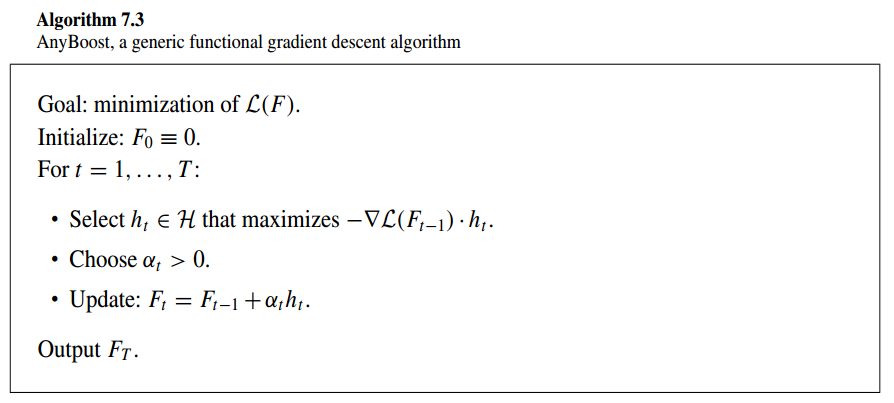
\includegraphics[scale = 0.4]{anyboost.png}}
\end{minipage}
\caption{\footnotesize{\textbf{A generic boosting algorithm based on functional gradient descent \citep{hastie2009elements}}}}
\label{fig: grad_boost}
\end{figure}

\item This step is close to the classical \emph{gradient descent algorithm} for \emph{(unconstrained) optimization}. \emph{\textbf{The major difference}} is that instead of computing \emph{the numerical gradient} $\nabla L$, we choose to \emph{\textbf{learn a new base hypothesis}} $h_t \in \cH$ that \emph{\textbf{matches}} the \emph{\textbf{negative functional gradient}}
\begin{align}
h_t := \arg\min_{h \in \cH}Diss(h_{\cD}, -\nabla L_{\cD}(F_{t-1}) ),  \label{eqn: functional_gradient_descent}
\end{align} where $Diss$ is some \emph{\textbf{distance/dissimilarity measure}} between two functions on given data set $\cD$. Thus the new base hypothesis $h_t$ plays role of $-\nabla L(F_{t-1})$ and it is then merging with existing function $F_{t-1}$ to \emph{make corrections}.

\item It can be shown that for AdaBoost, the loss functional is the exponential loss:
\begin{align}
L(F)  \equiv L(y, F) := \exp\paren{- y F(x)} \label{def: exp_loss}
\end{align} and the functional gradient 
\begin{align}
\nabla L_{\cD}(F_{t-1}) := \brac{\frac{-y_i \exp\paren{-y_i F_{t-1}(x_i)} }{m}}_{i=1\xdotx{,}m}. \label{eqn: adaboost_functional_gradient_on_samples}
\end{align} Choose similarity measure as \emph{the  cosine similarity}, which means that the goal is to optimize 
\begin{align*}
\max_{h \in \cH} S(h_{\cD}, -\nabla L_{\cD}(F_{t-1}) ) &= \max_{h \in \cH} \frac{1}{m}\sum_{i=1}^{m} y_i h_t(x_i)\exp\paren{-y_i F_{t-1}(x_i)} \\
&= \max_{h \in \cH}\sum_{i=1}^{m}D_{t}(i) y_i h_t(x_i) := 1- 2\epsilon_t
\end{align*} So the goal of the maximizing the cosine similarity is equivalent to minimizing the error rate $\epsilon_t$ on weighted sample distribution $\cD_t$. The hypothesis weight $\alpha_t$ is chosen to minimize the exponential loss \eqref{def: exp_loss}.

\end{itemize}

\subsection{Gradient Boost}
\begin{figure}
\begin{minipage}[t]{1\linewidth}
  \centering
  \centerline{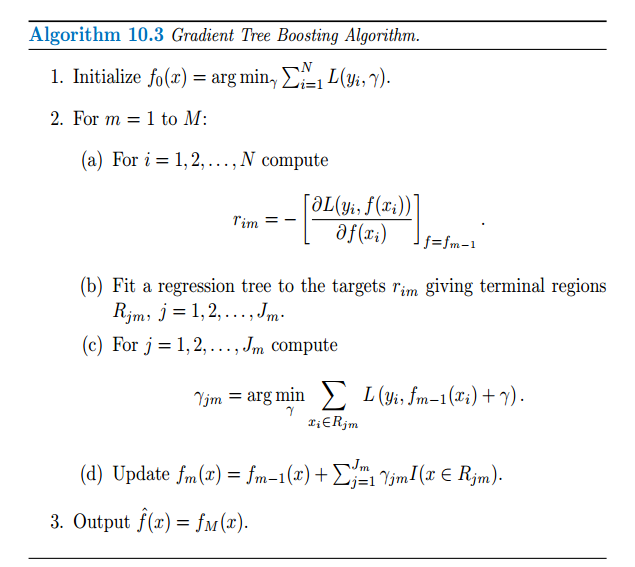
\includegraphics[scale = 0.5]{grad_boost.png}}
\end{minipage}
\caption{\footnotesize{\textbf{Gradient Boost Tree Algorithm \citep{hastie2009elements}}}}
\label{fig: grad_boost}
\end{figure}


\begin{itemize}
\item The interpretation of functional gradient descent can be used to develop a series of new boosting algorithms with different loss $L$ than exponential loss.

\item The \emph{\textbf{gradient boosting methods}} uses the negative functional gradient on samples $\cD$ as  
\begin{align}
-\nabla L_{\cD}(F_{t-1}) := -\brac{\partdiff{L(y, h)}{h_t(x_i)}\Bigr|_{h = F_{t-1}}}_{i=1\xdotx{,}m} \equiv \brac{r_{i,t}}_{i=1\xdotx{,}m} \label{eqn: grad_boost}
\end{align} 

\item At each iteration, it learns a base hypothesis that minimize \emph{the mean squared error loss}. In other word, it treats \emph{the negative functional gradient vector} $\brac{r_{i,t}}_{i=1}^{m}$ as \emph{the \underline{\textbf{residual}} and perform \underline{\textbf{regression tasks iteratively}}}. That is,
\begin{align}
\min_{h_t \in \cH} \sum_{i=1}^{m}\paren{r_{i,t} - h_t(x_i)}^2 = \min_{h_t \in \cH} \sum_{i=1}^{m}\norm{-\nabla L_{\cD}(F_{t-1}) - h_t}{2}^2 \label{eqn: grad_boost_regression_task}
\end{align}

\item Equivalently,  \emph{\textbf{the negative functional gradient}} becomes \emph{\textbf{the pseudo-label}} for the new hypothesis during the learning. 

\item Compared to \emph{AdaBoost}, \emph{\textbf{the Gradient Boost}} has several differences:
\begin{enumerate}
\item Gradient boost generalized the AdaBoost by \emph{choosing a \textbf{general loss function}} in the learning task, which could be more efficient and more \emph{\textbf{flexible}} for some tasks. 

\item Unlike AdaBoost, \underline{\emph{\textbf{no sample reweighting is needed for Gradient Boost}}} since the role of error rate $\epsilon_t$ and sample distribution $\cD_t$ is fulfilled by \emph{the functional gradient} $\nabla L_{\cD}(F_{t-1})$. In particular, \emph{\textbf{correctly labeled samples}} have \emph{\textbf{smaller functional gradients}} while \emph{\underline{\textbf{misclassified} samples have \textbf{larger functional gradients}}}.

In Gradient Boosting, `\emph{shortcomings}' (of existing weak learners) are identified by \emph{\textbf{gradients}}. In \emph{AdaBoost}, `\emph{shortcomings}' are identified by \emph{high-weight data points}.
\end{enumerate}

\item It tends to say that the main differences are that \emph{Gradient Boosting is a \underline{\textbf{generic algorithm}} to \textbf{find approximate solutions} to \textbf{the additive modeling problem}}, while AdaBoost can be seen as a special case with a particular loss function. Hence, \emph{Gradient Boosting is \textbf{much more flexible}}.

However, as pointed by Freund and Schapire \citep{schapire2012boosting}, \emph{\textbf{optimizing the exponential loss alone cannot explain the performance of AdaBoost}}. It is likely due to \emph{\textbf{large margin property}} and \emph{\textbf{the adversarial training procedure}} that the AdaBoost outperforms its counterpart in optimization only approach. It is critical to take into account \emph{the particular \textbf{dynamics} of the algorithm}, not just the objective function.
\end{itemize}

\section{Theoretical Guarantee for Boosting}
\begin{itemize}
\item \begin{remark} (\emph{\textbf{Data}})\\
Define an \emph{\textbf{observation}} as a $d$-dimensional vector $x$. The \emph{unknown} nature of the observation is called a \emph{\textbf{class}}, denoted as $y$. The domain of observation is called an \emph{\textbf{input space} or \textbf{feature space}}, denoted as $\cX\subset \bR^{d}$, whereas the domain of class is called the \emph{\textbf{target space}}, denoted as $\cY$. For \emph{\textbf{classification task}}, $\cY= \set{1,\ldots, M}$; and for \emph{\textbf{regression task}}, $\cY = \bR$.   A \emph{\textbf{concept}} $c: \cX \rightarrow \cY$ is the \emph{input-output association} from the nature and is \emph{to be learned} by \emph{\textbf{a learning algorithm}}.  Denote $\cC$ as \emph{the set of all concepts} we wish to learn as the \emph{\textbf{concept class}}. The learner is requested to output a \emph{prediction rule}, $h : \cX \to \cY$. This function is also called a \emph{\textbf{predictor}}, a \emph{\textbf{hypothesis}}, or a \emph{\textbf{classifier}}. The predictor can be used to predict the label of new domain points.  Denote a collection of $n$ \emph{\textbf{samples}} as 
\begin{align*}
\cD \equiv \cD_n = \paren{(X_1, Y_1) \xdotx{,} (X_n, Y_n)} \equiv  \paren{(X_1, c(X_1)) \xdotx{,} (X_n, c(X_n))} .
\end{align*} Note that $\cD_n$ is a finite \emph{\textbf{sub-sequence}} in $(\cX \times \cY)^n$.
\end{remark}

\item \begin{definition} (\emph{\textbf{Generalization Error in Deterministic Scenario}})  \citep{mohri2018foundations}\\
Under \emph{a deterministic scenario}, \underline{\emph{\textbf{generalization error}}} or the \underline{\emph{\textbf{risk}}} or simply \underline{\emph{\textbf{error}}} for the \emph{classifier} $h \in \cH$ is defined as
\begin{align}
L(h) \equiv L_{\cP, c}(h)  &= \cP\set{h(X) \neq c(X)} \equiv \E{X}{\ind{h(X)\neq c(X)}}\label{expr: gen_err_determin}
\end{align}
with respect to the concept $c \in \cC$ and \emph{the feature distribution} $\cP \equiv \cP_X$.
\end{definition}

\item 
\begin{definition} (\emph{\textbf{Empirical Error or Training Error}}) \\
Given the data $\cD$, the \emph{\textbf{training error}} or \underline{the \emph{\textbf{empirical error/risk}}} of a hypothesis $h \in \cH$ is defined as 
\begin{align*}
\widehat{L}(h)   \equiv \widehat{L}_{\cD}(h)  &= \frac{1}{n}\sum_{i=1}^{n}\ind{h(X_i)\neq Y_i} = \frac{1}{n}\abs{\set{i: h(X_i)\neq Y_i}} := \Em{}{\ind{h(X) \neq Y}}
\end{align*} where either $Y = c(X)$ or $Y$ is a random variable associated with $X$.
\end{definition}

\item \begin{definition}(\emph{\textbf{The Realizable Assumption}})\\
There exists $h^{*} \in \cH$ s.t. $L_{\cP, c}(h^{*}) = 0.$
\end{definition}

\item \begin{definition}(\textbf{\emph{PAC Learnability}})\\
A hypothesis class $\cH$ is \underline{\textbf{\emph{PAC learnable}}} if there exist a function $m_{\cH}: (0,1)^2 \to \bN$ and a learning algorithm with the following property: For every $\epsilon, \delta \in (0,1)$, \emph{for every distribution $\cP$ over $\cX$}, and \emph{for every labeling function $c: \cX \to \set{0,1}$}, if \emph{the realizable assumption} holds with respect to $\cH$, $\cP$, $c$, then when running the learning algorithm on $m \ge m_{\cH}(\epsilon, \delta)$ i.i.d. examples generated by $\cP$ and labeled by $c$, the algorithm returns a hypothesis $h$ such that, with probability of at least $1- \delta$ (over the choice of the examples), 
\begin{align*}
L_{\cP, c}(h) \le \epsilon.
\end{align*}
\end{definition}
\end{itemize}
\subsection{Weak Learner}
\begin{itemize}
\item  \begin{definition}(\textbf{\emph{$\gamma$-Weak Learnability}})  \citep{schapire2012boosting, shalev2014understanding} \\
A learning algorithm, $\cA$, is a \underline{\textbf{\emph{$\gamma$-weak-learner}}} for a class $\cH$ if there exists a function  $m_{\cH}: (0,1) \to \bN$ such that for \emph{\textbf{every}} $\delta \in (0,1)$, \emph{\textbf{for every distribution} $\cP$ over $\cX$}, and \emph{\textbf{for every labeling function}} $c: \cX \to \set{-1, +1}$, if \emph{the realizable assumption  holds} with respect to $\cH$, $\cP$, $c$, then when running the learning algorithm on $m \ge m_{\cH}(\delta)$ i.i.d. examples generated by $\cP$ and labeled by $c$, the algorithm returns a hypothesis $h$ such that, with probability of at least $1- \delta$,
\begin{align*}
L_{\cP, c}(h) \le \frac{1}{2}  - \gamma.
\end{align*} A hypothesis class $\cH$ is \underline{\textbf{\emph{$\gamma$-weak-learnable}}} if there exists a \emph{$\gamma$-weak-learner} for that class.
\end{definition}

\item \begin{remark}
We call PAC learnalbe \emph{\textbf{the strong learnable}}.
\end{remark}

\item \begin{remark} (\textbf{\emph{Weak Learner Without Accuracy Guarantee}})\\
Unlike \emph{the PAC learner}, who guarantees that \emph{with high probability} the generalization error rate is less than $\epsilon$ \emph{\textbf{for all $\epsilon$}}, a \emph{\textbf{$\gamma$-weak-learner}} guarantees that with high probability, the error rate is less than $\epsilon$ \underline{\textbf{\emph{for some}} $\epsilon = 1/2 - \gamma$}, i.e. \emph{less than half with a margin $\gamma$}.

In other word, \emph{under the realizablity assumption}, it is expected that \textit{\textbf{with more data}}, \emph{\textbf{a PAC learner}} can learn the ``\emph{true}" labeling function behind the data, (i.e. \emph{\textbf{zero generalization error}} with high probability). While a \emph{\textbf{$\gamma$-weak-learner}} can only get \emph{\textbf{slightly better than random guess}} and it is \emph{\textbf{not} expected to have \textbf{lower error rate}} even if more data are available.
\end{remark}

\item \begin{remark} (\textbf{\emph{Weak Learner is as Hard as PAC Learner}})\\
\emph{The fundamental theorem of learning}  states that if a hypothesis class $\cH$ has a VC dimension $d$, then \emph{the sample complexity of PAC learning $\cH$} satisfies $m_{\cH}(\epsilon, \delta) \ge  C_1 (d+\log(1/\delta))/\epsilon$, where $C_1$ is a constant. Applying this with $\epsilon = 1/2 - \gamma$ we immediately obtain that \emph{\textbf{if $d = \infty$ then $\cH$ is not $\gamma$-weak-learnable}}. 

This implies that from \emph{\textbf{the statistical perspective}} (i.e., if we ignore \emph{computational complexity}), \emph{\underline{\textbf{weak learnability} is also characterized by the VC dimension of $\cH$} and therefore is just \underline{\textbf{as hard as PAC (strong) learning}}}. However, when we do consider \emph{\textbf{computational complexity}}, the potential advantage of weak learning is that maybe there is \emph{an algorithm that satisfies the requirements of weak learning and \textbf{can be implemented efficiently}}.
\end{remark}
\end{itemize}
\subsection{Training Error Bounds}
\begin{itemize}
\item \begin{remark}
Recall that $h_t \in \cH$ are base learners for $t \in [1,T]$, and $(\alpha_1 \xdotx{,} \alpha_{T}) \in \Sigma_{T}$. The \emph{combined learner} is
\begin{align*}
H(x) := \sgn{\sum_{t=1}^{T}\alpha_t h_t(x)}
\end{align*}
\end{remark}

\item The space of all such combined classifiers is defined as below:
\begin{definition}(\textbf{\emph{Ensemble Hypothsis Class}})\\
Define the class of $T$ \emph{\textbf{linear combinations of base hypotheses}} from $\cH$ as
\begin{align}
L(\cH, T) &:=  \set{\sgn{\sum_{t=1}^{T}\alpha_t h_t(\cdot )}:  \alpha \in \bR^{T},  h_t \in \cH,  t = 1\xdotx{,} T }  \label{def: linear_ensemble_class}
\end{align}
\end{definition}

\item \begin{definition}(\textbf{\emph{Linear Threshold Functions}})\\
Define $\Sigma_n$  as the space of all \underline{\textbf{\emph{linear threshold functions}}}
\begin{align*}
\Sigma_n := \set{\sgn{\inn{w}{x}}:  w \in \bR^n}.
\end{align*} Thus $L(\cH, T) = \set{\sigma\paren{h_1(x) \xdotx{,} h_{T}(x)} : \sigma \in \Sigma_{T}}$
\end{definition}



\item \begin{proposition}\label{prop: training_error_bound} (\textbf{Training Error Bound for AdaBoost}) \citep{schapire2012boosting}\\
Given the notation of Adaboost algorithm, let $\gamma_t = 1/2 - \epsilon_t$, and let $\cD_1$ be an arbitrary initial distribution over the training set. Then \textbf{the weighted training error} of the combined classifier $\cH$ with respect to $\cD_1$ is bounded as
\begin{align}
\widehat{L}_{\cD_1}(H) \le \prod_{t=1}^{T} \sqrt{1 - 4 \gamma_t^2} \le \exp\paren{- 2 \sum_{t=1}^{T}\gamma_t^2}. \label{ineqn: boosting_training_error_bound}
\end{align} 
\end{proposition}
\begin{proof}
Consider the linear combination of base classifiers:
\begin{align*}
f(x) := \sum_{t=1}^{T}\alpha_t h_t(x).
\end{align*} By definition of distribution $\cD_T$ via $\cD_{T-1}$ we have
\begin{align*}
\cD_{T+1}(i) &= \frac{ \exp\paren{-\alpha_T y_i h_T(x_i)}}{Z_T}\cD_{T-1}(i)  \\
&= \ldots\\
&= \frac{ \exp\paren{-\sum_{t=1}^{T}\alpha_t y_i h_t(x_i)}}{\prod_{t=1}^{T}Z_t}\cD_{1}(i) = \frac{ \exp\paren{- y_i f(x_i)}}{\prod_{t=1}^{T}Z_t} \cD_{1}(i)
\end{align*} Note that $H(x) \neq y$ if and only if $y f(x) < 0$, and $\mathds{1}_{(-\infty, 0]}(x) \le \exp(-x)$ so
\begin{align*}
\ind{H(x_i) \neq y_i} = \mathds{1}_{(-\infty, 0]}(y_i f(x_i)) \le \exp\paren{- y_i f(x_i)}.
\end{align*} By definition of training error, 
\begin{align}
\widehat{L}_{\cD_1}(H) &= \sum_{i=1}^{m}\ind{H(x_i) \neq y_i} \cD_1(i) \nonumber\\
&\le \sum_{i=1}^{m} \exp\paren{- y_i f(x_i)} \cD_1(i)  \nonumber\\
&=  \paren{\sum_{i=1}^{m} \cD_{T+1}(i)}\prod_{t=1}^{T}Z_t  \nonumber\\
&= \prod_{t=1}^{T}Z_t \label{pf: training_error_bound_1}
\end{align} Finally, by our choice of $\alpha_t = \frac{1}{2}\log\frac{1 - \epsilon_t}{\epsilon_t} = \frac{1}{2}\log\frac{1/2 + \gamma_t}{1/2 - \gamma_t}$, we have that
\begin{align}
Z_t &= \sum_{i=1}^{m}\cD_t(i)\exp\paren{-\alpha_t y_i h_t(x_i)} \nonumber\\
&= \exp\paren{-\alpha_t}\sum_{i: H(x_i) = y_i}\cD_t(i)  + \exp\paren{\alpha_t}\sum_{i: H(x_i) \neq y_i}\cD_t(i)  \nonumber\\
&= \exp\paren{-\alpha_t}(1 - \epsilon_t) + \exp\paren{\alpha_t}\epsilon_t \qquad (\text{by definition of error }\epsilon_t)  \nonumber\\
&= \exp\paren{-\alpha_t}(1/2 + \gamma_t) + \exp\paren{\alpha_t}(1/2 - \gamma_t) \qquad (\text{substitute }\alpha_t) \nonumber\\
&=\sqrt{\paren{1 - 2\gamma_t}\paren{1 +2 \gamma_t}} \label{pf: partition_fun_train_error}
\end{align} Substituting \eqref{pf: partition_fun_train_error} into \eqref{pf: training_error_bound_1}, we have the result. \qed
\end{proof}

\end{itemize}
\subsection{Generalization Error Bounds for Finite Hypothesis Class}
\begin{itemize}
\item \begin{definition} (\emph{\textbf{Restriction of $\cH$ to $\cD$}}). \\
Let $\cH$ be a class of functions from $\cX$ to $\set{0,1}$ and let $\cD = \set{x_1 \xdotx{,} x_m} \subset \cX$. 

\underline{\emph{\textbf{The restriction of $\cH$ to $\cD$}}} is \emph{the set of functions} from $\cD$ to $\set{0,1}$ that can be \emph{derived from} $\cH$. That is,
\begin{align*}
\cH_{\cD} := \set{(h(x_1) \xdotx{,} h(x_m)): h \in \cH},
\end{align*}
where we \emph{\textbf{represent}} each function from $\cX$ to $\set{0,1}$ as a \emph{\textbf{vector}} in $\set{0,1}^{\abs{\cD}}$.
\end{definition}

\item \begin{definition}(\emph{\textbf{Shattering}}). \\
A hypothesis class $\cH$ \underline{\emph{\textbf{shatters}} a finite set $\cD \subset \cX$} if \emph{\textbf{the restriction of $\cH$ to $\cD$}} is the set of \emph{\textbf{all functions}} from $\cD$ to $\set{0,1}$. That is, 
\begin{align*}
\abs{\cH_{\cD}} &= 2^{\abs{\cD}}.
\end{align*}
\end{definition}

\item \begin{definition} (\emph{\textbf{Growth Function}}). \\
Let $\cH$ be a hypothesis class. Then \underline{\emph{\textbf{the growth function of $\cH$}}}, denoted $\tau_{\cH}: \bN \to \cN$, is defined as
\begin{align*}
\tau_{\cH}(m) &:= \max_{\cD \subset \cX: \abs{\cD} = m}\abs{\cH_{\cD}}.
\end{align*}
In words, $\tau_{\cH}(m)$ is \textbf{\emph{the number of different functions}} from a set $\cD$ of \emph{\textbf{size $m$}} to $\set{0,1}$ that can be obtained by \emph{\textbf{restricting $\cH$ to $\cD$}}.
\end{definition}

\item \begin{lemma} (\textbf{Sauer's Lemma}). \citep{shalev2014understanding, mohri2018foundations}\\
Let $\cH$ be a hypothesis class with $VCdim(\cH) \le d < \infty$. Then, for all $m \ge d + 1$, 
\begin{align}
\tau_{\cH}(m) &\le \sum_{i=0}^{d}{{m}\choose{i}} \le \paren{\frac{em}{d}}^{d}.  \label{eqn: sauer_lemma}
\end{align}
\end{lemma}

\item 
\begin{proposition} \label{cor: generalization_bound_growth}   (\textbf{Generalization Bound via Growth Function})  \citep{mohri2018foundations}\\
Let $\cH$ be a family of functions taking values in $\set{-1, +1}$.  Then, for any $\delta > 0$, with probability at least $1 - \delta$, for any $h \in \cH$,
\begin{align}
L(h) \le \widehat{L}_{m}(h) + \sqrt{\frac{2 \log \tau_{\cH}(m)}{m}} +\sqrt{\frac{\log(1/\delta)}{2m}} \label{ineqn: generalization_bound_growth_number}
\end{align}
Growth function bounds can be also derived directly (without using Rademacher complexity bounds first). The resulting bound is then the following:
\begin{align}
\cP\set{\exists h\in \cH, \abs{L(h) - \widehat{L}_{m}(h)} > \epsilon }  \le 4\tau_{\cH}(2m)\;\exp\paren{-\frac{m\epsilon^2}{8}} \label{ineqn: generalization_bound_growth_number_2}
\end{align}
which only differs from \eqref{ineqn: generalization_bound_growth_number} by constants.
\end{proposition}



\item The following lemma shows that the VC dimension of $\Sigma_T$ is $T$.
\begin{lemma} \citep{schapire2012boosting, mohri2018foundations}\\
The space $\Sigma_n$ of \textbf{linear threshold functions} over $\bR^n$ 
\begin{align*}
\Sigma_n := \set{\sgn{\inn{w}{x}}:  w \in \bR^n}
\end{align*}
has \textbf{VC-dimension} $n$.
\end{lemma}

\item \begin{remark}
Note that the class $\Sigma_n$ is  \textbf{\emph{the class of half-spaces}} $\{\inn{w}{x}: w \in \bR^n\}$ whose VC dimension is $n$. 
\end{remark}

\item \begin{lemma} (\textbf{Growth Number of Ensemble Hypothesis Class, Finite Hypothesis Class}) \citep{schapire2012boosting, shalev2014understanding} \\
Assume $\cH$ is \textbf{finite}. Let $m \ge T \ge 1$. For any set $\cD$ of $m$ points, the number of dichotomies realizable by $L(\cH, T)$ is bounded as follows:
\begin{align}
\abs{L(\cH, T)_{\cD}} \le \tau_{L(\cH, T)}(m) \le \paren{\frac{em}{T}}^T \abs{\cH}^T.  \label{ineqn: growth_fun_ensemble_finite}
\end{align}
\end{lemma}
\begin{proof}
Consider a new sample $\cD' := \set{Z_1 \xdotx{,} Z_m}$ where
\begin{align*}
Z_i := \paren{h_1(X_i) \xdotx{,} h_T(X_i)}.
\end{align*} Given that the VC dimension of $\Sigma_T$ is $T$, the bound on the growth number becomes
\begin{align}
\abs{L(\cH, T)_{\cD'}} \le \paren{\frac{em}{T}}^T. \label{pf: growth_fun_finite_1}
\end{align} That is, for \emph{fixed} $h_1 \xdotx{,} h_T$, \emph{the number of dichotomies} defined by functions of the form $\sigma(h_1(x) \xdotx{,} h_T(x))$ for $\sigma \in T$ is bounded as in equation \eqref{pf: growth_fun_finite_1}. Since the number of choices for $h_1 \xdotx{,} h_T$ is equal to $\abs{\cH}^T$, and since for each one of these, the number of dichotomies is as in equation \eqref{pf: growth_fun_finite_1}, we thus obtain the bound stated in the lemma. \qed
\end{proof}

\item \begin{theorem}  (\textbf{Generalization Bound for AdaBoost, Finite Hypothesis}) \citep{schapire2012boosting}\\
Suppose \textbf{AdaBoost} is run for $T$ rounds on $m \ge T$ random examples, using base classifiers from a \textbf{finite space} $\cH$. Then, with probability at least $1 - \delta$, the combined classifier $H$ satisfies
\begin{align}
L_{\cP, c}(H) \le \widehat{L}_{m}(H) + \sqrt{\frac{2 T\paren{ \log \abs{\cH} + \log(em/T) }}{m}} +\sqrt{\frac{\log(1/\delta)}{2m}} \label{eqn: generalization_bound_growth_number_adaboost_finite}
\end{align} Furthermore, with probability at least $1 - \delta$, if $\cH$ is realizable with the training set (i.e. $\widehat{L}_{m}(h) \equiv 0$), then
\begin{align}
L_{\cP, c}(H) &\le \frac{2 T\paren{ \log \abs{\cH} + \log(2em/T) } + 2\log(2/\delta)}{m}. \label{eqn: pac_sample_complexity_finite_case_consistency}
\end{align}
\end{theorem}
\end{itemize}
\subsection{Generalization Error Bounds via VC Dimension}
\begin{itemize}
\item \begin{lemma} (\textbf{Growth Number of Ensemble Hypothesis Class, VC Class}). \citep{schapire2012boosting}\\
Assume $\cH$ has \textbf{finite VC-dimension} $d \ge 1$. Let $m \ge \max\{T, d\} \ge 1$. For any set $\cD$ of $m$ points, the number of dichotomies realizable by $L(\cH, T)$ is bounded as follows:
\begin{align}
\abs{L(\cH, T)_{\cD}} \le \tau_{L(\cH, T)}(m) \le \paren{\frac{em}{T}}^T \paren{\frac{em}{d}}^{dT}.  \label{ineqn: growth_fun_ensemble_infinite}
\end{align}
\end{lemma}

\item \begin{lemma} (\textbf{VC-Dimension of Ensemble Hypothesis Class, VC Class}). \citep{schapire2012boosting, shalev2014understanding}\\
Assume $\cH$ has \textbf{finite VC-dimension} $\nu(\cH) = d$ and $\min\set{T, d} \ge 3$. Then the VC dimension of combined hypothesis class is bounded by
\begin{align}
\nu(L(\cH, T)) \le T\paren{d + 1}\paren{3\log\paren{T(d+1)} + 2} = \cO(Td \log(Td)).  \label{ineqn: vc_dim_ensemble_infinite}
\end{align}
\end{lemma}

\item \begin{remark}(\textbf{\emph{Lower Bound on VC Dimension}}). \citep{shalev2014understanding}\\
For some base hypothesis class $\cH$, the VC-dimension of ensemble is at least $Td$. For instance, for $\cH_n$  be the class of \emph{decision stumps} over $\bR^n$,  we can show that $\log(n) \le d = \nu(\cH) \le 2\log(n) + 5$.  In this example, for all $T \ge 1$, 
\begin{align*}
\nu(L(\cH_n, T)) \ge 0.5T\log(n) \asymp \Omega\paren{Td}.
\end{align*} 
\end{remark}

\item \begin{theorem} \label{thm: growth_fun_adaboost}  (\textbf{Generalization Bound for AdaBoost via VC Dimension}). \citep{schapire2012boosting}\\
Suppose \textbf{AdaBoost} is run for $T$ rounds on $m \ge \max\{T, d\}$ random examples, using base classifiers from a \textbf{finite space} $\cH$. Then, with probability at least $1 - \delta$, the combined classifier $H$ satisfies
\begin{align}
L_{\cP, c}(H) \le \widehat{L}_{m}(H) + \sqrt{\frac{2 T\paren{ d\log(em/d) + \log(em/T) }}{m}} +\sqrt{\frac{\log(1/\delta)}{2m}} \label{ineqn: generalization_bound_growth_number_adaboost}
\end{align} Furthermore, with probability at least $1 - \delta$, if $\cH$ is realizable with the training set (i.e. $\widehat{L}_{m}(h) \equiv 0, \forall h\in \cH$), then
\begin{align}
L_{\cP, c}(H) &\le \frac{2 T\paren{ d\log(2em/d) + \log(2em/T) } + 2\log(2/\delta)}{m}. \label{ineqn: pac_sample_complexity_consistency}
\end{align}
\end{theorem}

\item \begin{remark}(\emph{\textbf{Limit of VC Dimension Analysis}})\\
The upper bound grows as $\cO(dT \log(dT))$, thus the bound suggests that \emph{\textbf{AdaBoost} could \textbf{overfit} for \textbf{large values of $T$}}, and indeed this can occur. See Figure \ref{fig: overfitting_adaboost}. However, in many cases, it has been observed empirically that \emph{the generalization error of AdaBoost \textbf{decreases}} as a function of \emph{the number of rounds} of boosting $T$.
\end{remark}

\begin{figure}
\begin{minipage}[t]{1\linewidth}
  \centering
  \centerline{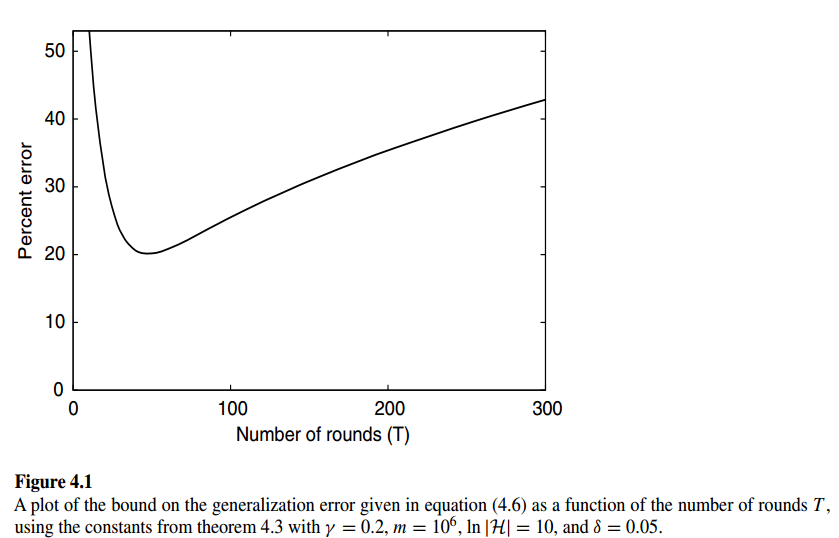
\includegraphics[scale = 0.4]{overfitting_adaboost.png}}
\end{minipage}
\caption{\footnotesize{\textbf{AdaBoost may overfit if the number of rounds $T$ is too large. \citep{schapire2012boosting}}}}
\label{fig: overfitting_adaboost}
\end{figure}


\item \begin{corollary}  \citep{schapire2012boosting}\\
Assume, in addition to the assumptions of theorem \ref{thm: growth_fun_adaboost}, that each base classifier has weighted error $\epsilon_t \le 1/2 - \gamma$ for some $\gamma > 0$. Let the number of rounds $T$ be equal to
\begin{align*}
\inf\set{T \in \bN: T \ge \frac{\log(m)}{2\gamma^2}}
\end{align*} Then, with probability at least $1 - \delta$, the generalization error of the combined classifier $H$ will be at most
\begin{align*}
\cO\paren{\frac{1}{m}\brac{\frac{\log(m)}{\gamma^2}\paren{\log(m) + d\log\paren{\frac{m}{d}}} + \log\paren{\frac{1}{\delta}}}}
\end{align*}
\end{corollary}

\item \begin{remark}
Ignoring the log factor, the generalization error bound \eqref{ineqn: generalization_bound_growth_number_adaboost} can be summarized as
\begin{align*}
L_{\cP, c}(H) \le \widehat{L}_{m}(H) + \cO\paren{\sqrt{\frac{T \cC_{\cH}}{m}}}
\end{align*} where $\cC_{\cH}$ is some complexity measure of base class $\cH$.
\end{remark}

\item \begin{theorem} (\textbf{Strong Learnable $\Leftrightarrow$ Weak Learnable})  \citep{schapire2012boosting}\\
A target class $\cH$ is (efficiently) \textbf{weakly} PAC learnable \textbf{if and only if} it is (efficiently) \textbf{strongly} PAC learnable.
\end{theorem}
\end{itemize}

\subsection{Generalization Error Bounds via  Margin Theory}
\begin{itemize}

\item \begin{definition} (\textbf{\emph{$L_1$-Margin}}) \citep{mohri2018foundations, schapire2012boosting}\\
\underline{\emph{\textbf{The $L_1$-margin}}} $\rho(x)$ of a point $x \in \cX$ with label $y \in \set{-1, +1}$ for \emph{a linear combination of base classifiers} $g = \sum_{t=1}^{T}\alpha_t h_t = \inn{\alpha}{h}$ with $\alpha \neq 0$ and $h_t \in \cH$ for all $t \in [1, T]$ is defined as
\begin{align}
\rho(x) := y \frac{\inn{\alpha}{h(x)}}{\norm{\alpha}{1}} =  \frac{\sum_{t=1}^{T}\alpha_t y h_t(x)}{\norm{\alpha}{1}} \label{def: l1_margin}
\end{align} \underline{\emph{\textbf{The $L_1$-margin}}} of a linear combination classifier $g$ \emph{\textbf{with respect to a sample}} $\cD$ is \emph{\textbf{the minimum margin} of the points within the sample}:
\begin{align}
\rho := \min_{i=1\xdotx{,} m}y_i \frac{\inn{\alpha}{h(x_i)}}{\norm{\alpha}{1}} = \min_{i=1\xdotx{,} m} \frac{\sum_{t=1}^{T}\alpha_t y_i  h_t(x_i)}{\norm{\alpha}{1}} \label{def: l1_margin_sample}
\end{align}
\end{definition}

\item \begin{definition}(\textbf{\emph{Margin Loss Function}})  \citep{mohri2018foundations, schapire2012boosting}\\
For any $\rho > 0$,  \underline{\emph{\textbf{the $\rho$-margin loss}}} $L_{\rho}: \bR \times \bR \to \bR_{+}$ is defined for all $y, y' \in \bR$ by  $L_{\rho}(y,y') = \varphi_{\rho}(yy')$ where $\varphi$ is defined as a piecewise-linear function,
\begin{align*}
\varphi_{\rho}(x) &:= \left\{ \begin{array}{cc}
1 &\text{if } x\le 0\\
1 - x/\rho &\text{if } 0 \le x \le \rho\\
0 &\text{if } x \ge \rho
\end{array}
\right.
\end{align*} This function is \textbf{\emph{Lipschitz}} with $L_{\varphi} = 1/\rho$.
\end{definition}

\begin{figure}
\begin{minipage}[t]{1\linewidth}
  \centering
  \centerline{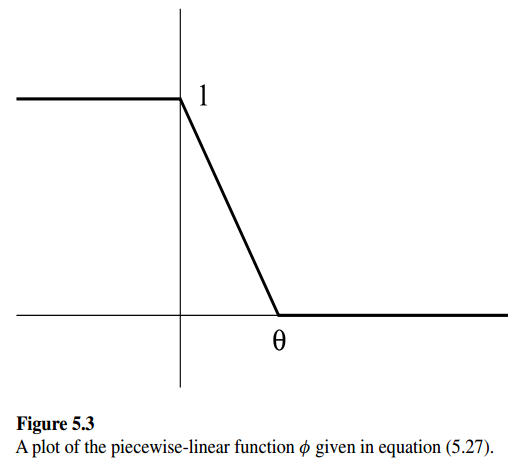
\includegraphics[scale = 0.4]{piecewise_linear.png}}
\end{minipage}
\caption{\footnotesize{\textbf{The piecewise linear function $\varphi_{\phi}$. \citep{schapire2012boosting}}}}
\label{fig: piecewise_linear}
\end{figure}


\item \begin{definition}(\textbf{\emph{Empirical Margin Loss}}) \citep{schapire2012boosting, mohri2018foundations}
Given a sample $\cD_m$ and a hypothesis $h$, \underline{\emph{\textbf{the empirical margin loss}}} is defined by
\begin{align}
\widehat{L}_{m, \rho}(h)&=  \frac{1}{m}\sum_{i=1}^{m}\varphi_{\rho}\paren{Y_i h(X_i)}  \label{eqn: emp_margin_loss}
\end{align} Note that for any $i \in [1, m]$, $\ind{y_i h(x_i) \le 0}\le \varphi_{\rho}\paren{y_i h(x_i)} \le \ind{y_i h(x_i) \le \rho}$. Thus, the empirical margin
loss can be bounded as follows:
\begin{align}
\widehat{L}(h) &= \frac{1}{m}\sum_{i=1}^{m}\ind{h(X_i)\neq Y_i}  = \frac{1}{m}\sum_{i=1}^{m}\ind{Y_i h(X_i) \le 0} \nonumber \\
&\le \widehat{L}_{m, \rho}(h) \le  \frac{1}{m}\sum_{i=1}^{m}\ind{Y_i h(X_i) \le \rho}. \label{eqn: emp_margin_loss_bound}
\end{align}
\end{definition}

\item \begin{remark}
In all the results that follow, the empirical margin loss can be replaced by this upper bound, which admits a simple interpretation: it is \emph{the fraction of the points in the training sample $\cD$ that have been \textbf{misclassified} or classified \textbf{with confidence less than} $\rho$}. 
\end{remark}

\item \begin{remark}
When the coefficients $\alpha_t$ are \emph{\textbf{non-negative}}, as in the case of \emph{AdaBoost}, $\rho(x)$ is \emph{\textbf{a convex combination}} of the base classifier values $h_t(x)$. In particular, if the base classifiers $h_t$ take values in $[-1, +1]$, then $\rho(x)$ is in $[-1, +1]$. \emph{The absolute value} $\abs{\rho(x)}$ can be interpreted as \emph{\textbf{the confidence} of the classifier} $g$ in that label.
\end{remark}

\item \begin{definition}(\emph{\textbf{Convex Hull of Hypothesis Class}})\\
For any hypothesis class $\cH$, \underline{\textbf{\emph{the convex hull}}} of set $\cH$, denoted as $\text{conv}(\cH)$, is defined as 
\begin{align*}
\text{conv}(\cH) := \set{\sum_{k=1}^{T}\lambda_k h_k(\cdot):  T \ge 1, \forall k \in [1, T], \lambda_k \ge 0, h_k \in \cH, \sum_{k=1}^{T}\lambda_k = 1}.
\end{align*}
\end{definition}

\item \begin{remark}
Let $\cH$ be our space of base classifiers, and let $\cM$ be the space of all ``\emph{\textbf{margin functions}}" of the form $yf(x)$ where $f$ is any convex combination of base classifiers:
\begin{align*}
\cM := \set{(x,y) \to yf(x): f \in  \text{conv}(\cH)}
\end{align*} Note that $\widehat{\frR}_{\cD}(\cM)  = \widehat{\frR}_{\cD}(\text{conv}(\cH))$ since $y_i \sigma_i$ has the same distribution as $\sigma_i$.
\end{remark}

\item \begin{definition} (\emph{\textbf{Empirical Rademacher Complexity}})\\
Let $\cG$ be a family of functions mapping from $\cZ := \cX \times \cY$ to $[a, b]$ and $\cD = (z_1 \xdotx{,} z_n)$ a fixed \emph{sample} of size $n$ with elements in $\cZ$. Then, \underline{\emph{\textbf{the empirical Rademacher complexity}}} of $\cG$ \emph{with respect to the sample $\cD$} is defined as:
\begin{align}
\widehat{\mathfrak{R}}_{\cD}(\cG)&= \E{\sigma}{\sup_{g \in \cG}\frac{1}{n}\sum_{i=1}^{n}\sigma_{i}g(z_i)}   \label{eqn: rademacher_complexity}
\end{align}
where $\sigma := (\sigma_1 \xdotx{,} \sigma_n)$ are  \textbf{\emph{independent uniform random variables}} taking values in $\set{-1, +1}$. The random variables $\sigma_i$ are called \underline{\emph{\textbf{Rademacher variables}}}.
\end{definition}




\item \begin{proposition}(\textbf{Empirical Rademacher Complexity of a Convex Hull of Function Class}\\
Let $\cH$ be a set of functions mapping from $\cX$ to $\bR$. Then, for any sample $\cD$, the empirical Rademacher complexity 
\begin{align}
\widehat{\frR}_{\cD}(\text{conv}(\cH))  = \widehat{\frR}_{\cD}(\cH) \label{eqn: rademacher_complexity_convex_hull}
\end{align} where $\text{conv}(\cH)$ is \textbf{the convex hull} of set $\cH$.
\end{proposition}

\item \begin{theorem} (\textbf{Uniform Bound via Rademacher Complexity}) \citep{mohri2018foundations}\\
Let $\cG$ be a family of functions mapping from $\cZ$ to $[0, 1]$. Then, for any $\delta > 0$, \textbf{with probability at least} $1 - \delta$, each of the following holds for all $g \in \cG$:
\begin{align}
\E{}{g(Z)} &\le \frac{1}{m}\sum_{i=1}^{m}g(Z_i) + 2 \frR_{m}(\cG)  + \sqrt{\frac{\log(1 / \delta)}{2m}} \label{ineqn: Rademacher_bound_1}
\end{align}
and
\begin{align}
\E{}{g(Z)} &\le \frac{1}{m}\sum_{i=1}^{m}g(Z_i) + 2 \widehat{\mathfrak{R}}_{m}(\cG) + 3\sqrt{\frac{\log(2 / \delta)}{2m}} \label{ineqn: Rademacher_bound_2}
\end{align}
\end{theorem}


\item Based on the theorem above, we can have the generalization error bound via margin:
\begin{theorem} (\textbf{Ensemble Rademacher Margin Bound})  \citep{schapire2012boosting, mohri2018foundations} \\
Let $\cH$ denote a set of real-valued functions. Fix $\rho > 0$. Then, for any $\delta > 0$, with
probability at least $1 - \delta$, each of the following holds for all $h \in \text{conv}(\cH)$:
\begin{align}
L(h) &\le \widehat{L}_{m, \rho}(h) + \frac{2}{\rho} \frR_{m}(\cH)  + \sqrt{\frac{\log(1 / \delta)}{2m}} \label{ineqn: Rademacher_margin_bound}\\
L(h) &\le \widehat{L}_{m, \rho}(h)  +  \frac{2}{\rho} \widehat{\mathfrak{R}}_{m}(\cH) + 3\sqrt{\frac{\log(2 / \delta)}{2m}}  \label{ineqn: Rademacher_margin_bound_2}
\end{align}
\end{theorem}
\begin{proof}
Consider the family of functions taking values in $[0, 1]$:
\begin{align*}
\varphi_{\rho} \circ \cM := \set{\varphi_{\rho} \circ f:  f\in \cM}
\end{align*} where $\cM := \set{(x,y) \to yh(x): h \in  \text{conv}(\cH)}$. By the generalization bound via Rademacher complexity,
\begin{align*}
\E{}{\varphi_{\rho}(Y h(X))} &\le \frac{1}{m}\sum_{i=1}^{m}\varphi_{\rho}\paren{Y_i h(X_i)} + 2 \frR_{m}(\varphi_{\rho} \circ \cM )  + \sqrt{\frac{\log(1 / \delta)}{2m}}
\end{align*} By inequality \eqref{eqn: emp_margin_loss_bound}
\begin{align*}
L(h) =\E{}{\ind{Y \neq h(X)}} \le \E{}{\varphi_{\rho}(Y h(X))}
\end{align*} thus
\begin{align*}
L(h)  &\le \widehat{L}_{m, \rho}(h) + 2 \frR_{m}(\varphi_{\rho} \circ \cM )  + \sqrt{\frac{\log(1 / \delta)}{2m}}
\end{align*}
Note that $\varphi_{\rho}$ is $(\frac{1}{\rho})$-Lipschitz function. 
\begin{align*}
\frR_{m}(\varphi_{\rho} \circ \cM ) &\le  \frac{1}{\rho}\frR_{m}( \cM ) &&\quad  (\text{ by contraction principle})\\
&= \frac{1}{\rho}\frR_{m}(\text{conv}(\cH) ) &&\quad  (\text{ since $y_i$ is absorbed by $\sigma_i$})\\
&= \frac{1}{\rho}\frR_{m}(\cH). &&\quad  (\text{ by \eqref{eqn: rademacher_complexity_convex_hull}})
\end{align*} This complete the proof. \qed
\end{proof}

\item \begin{theorem} (\textbf{Ensemble VC-Dimension Margin Bound}) \citep{schapire2012boosting, mohri2018foundations} \\
Let $\cH$ be a family of functions taking values in $\set{+1, -1}$ with VC-dimension $d$. Fix $\rho > 0$. Then, for any $\delta > 0$, with probability at least $1 - \delta$,  the following holds for all $h \in \text{conv}(\cH)$:
\begin{align}
L(h) &\le \widehat{L}_{m, \rho}(h) + \frac{2}{\rho}\sqrt{\frac{2d \log(em/d)}{m}}   + \sqrt{\frac{\log(1 / \delta)}{2m}} \label{eqn: Rademacher_margin_bound_vc_dim}
\end{align}
\end{theorem}

\item \begin{remark}
Note that from the point of view of binary classification, $g$ and $g/\norm{\alpha}{1}$ are equivalent since $\sgn{g} = \sgn{g/\norm{\alpha}{1}}$, thus $L(g) = L(g/\norm{\alpha}{1})$, but their empirical margin loss are distinct. Let $g =\sum^T_{t=1}\alpha_t h_t$ denote the function defining the classifier returned by AdaBoost after $T$ rounds of boosting when trained on sample $\cD$. Then, in view of \eqref{ineqn: Rademacher_margin_bound},  for any $\delta > 0$, with
probability at least $1 - \delta$
\begin{align}
L(g) &\le \widehat{L}_{m, \rho}(g/\norm{\alpha}{1}) + \frac{2}{\rho} \frR_{m}(\cH)  + \sqrt{\frac{\log(1 / \delta)}{2m}}  \label{ineqn: Rademacher_margin_bound_norm_l1}
\end{align}
\end{remark}

\item \begin{remark}(\textbf{\emph{Generalization Guarantee by Large Margin Only}})\\
Remarkably, \emph{\textbf{the number of rounds of boosting} $T$ \textbf{does not appear} in the generalization bound} \eqref{ineqn: Rademacher_margin_bound_norm_l1}. The bound depends only on \emph{the margin $\rho$, the sample size $m$, and the Rademacher complexity of the family of base classifiers $\cH$}. Thus, the bound guarantees an effective generalization if the margin loss $\widehat{L}_{m, \rho}(g/\norm{\alpha}{1})$ is small for a relatively large
$\rho$. 
\end{remark}


\begin{figure}
\begin{minipage}[t]{1\linewidth}
  \centering
  \centerline{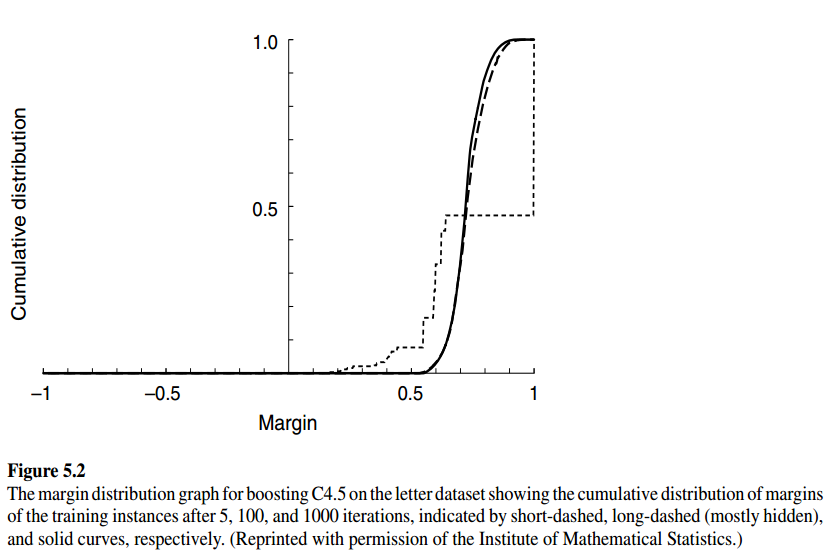
\includegraphics[scale = 0.4]{dist_margin.png}}
\end{minipage}
\caption{\footnotesize{\textbf{Distribution of margin for AdaBoost on one example dataset. \citep{schapire2012boosting}}}}
\label{fig: dist_margin}
\end{figure}

\item \begin{proposition} (\textbf{Empirical Margin Loss Bound for AdaBoost})  \citep{schapire2012boosting, mohri2018foundations} \\
Let $f =\sum^T_{t=1}\alpha_t h_t$ denote the function defining the classifier returned by AdaBoost after $T$ rounds of boosting and assume for all $t \in [1, T]$ that $\epsilon_t < 1/2$, which implies $\alpha_t > 0$. Then, for any $\rho > 0$, the following holds:
\begin{align}
\widehat{L}_{m, \rho}(f)  &\le  2^T\prod_{t=1}^{T}\sqrt{\epsilon_t^{1-\rho}(1 - \epsilon_t)^{1 + \rho}} \le \brac{(1- 2\gamma)^{1-\rho}(1+2\gamma)^{1+\rho}}^{T/2} \label{ineqn: emp_margin_loss_bound}
\end{align} where $ \gamma \le 1/2 - \epsilon_t$ for all $t$. Note that $\gamma > 0$ so $\brac{(1- 2\gamma)^{1-\rho}(1+2\gamma)^{1+\rho}} < 1$.
\end{proposition}
\begin{proof}
Consider the linear combination of base classifiers:
\begin{align*}
f(x) := \sum_{t=1}^{T}\alpha_t h_t(x).
\end{align*} Note that $y f(x) \le \rho$ if and only if
\begin{align*}
y \sum_{t=1}^{T}\alpha_t h_t(x) \le \rho \sum_{t=1}^{T}\alpha_t.
\end{align*} This implies that 
\begin{align*}
\exp\paren{- y \sum_{t=1}^{T}\alpha_t h_t(x) + \rho \sum_{t=1}^{T}\alpha_t} \ge 1 \ge \ind{y f(x) \le \rho}
\end{align*} Thus
\begin{align*}
\widehat{L}_{m, \rho}(f) = \frac{1}{m}\sum_{i=1}^{m}\ind{y_i f(x_i) \le \rho} &\le \exp\paren{\rho \sum_{t=1}^{T}\alpha_t}\brac{\frac{1}{m}\sum_{i=1}^{m}\exp\paren{- y_i \sum_{t=1}^{T}\alpha_t h_t(x_i)}}\\
&= \exp\paren{\rho \sum_{t=1}^{T}\alpha_t} \paren{\prod_{t=1}^{T}Z_t}  \quad \text{(See proof in Proposition \ref{prop: training_error_bound})}
\end{align*} Plugging in the values of $\alpha_t = \frac{1}{2}\log\frac{1- \epsilon_t}{\epsilon_t}$ and $Z_t = 2\sqrt{\epsilon_t(1-\epsilon_t)}$ and the derivation follows the same as in Proposition \ref{prop: training_error_bound}, which gives the final result. \qed
\end{proof} 

\item \begin{remark}
This bound implies that the fraction of training examples with $yf(x) \le \rho$ decreases to zero \emph{\textbf{exponentially fast}} with $T$, and must actually be equal to zero at some point since this fraction must always be a multiple of $1/m$.
\end{remark}

\item \begin{remark} (\emph{\textbf{AdaBoost Maximize the Margin? }})\\
The margin bounds combined with the bound on the empirical margin loss suggest that under some conditions, \emph{\textbf{AdaBoost} can achieve \textbf{a large margin on the training sample}}. They could also serve as a theoretical explanation of the empirical observation that \emph{in some tasks \textbf{the generalization error decreases} as a function of $T$ even after the error on the training sample is zero}: \emph{the margin would continue to increase}. 

But does \emph{AdaBoost} maximize the $L_1$-margin? \emph{\textbf{No}}. It has been shown that \emph{AdaBoost may \textbf{converge to a margin} that is \textbf{significantly smaller than the maximum margin}}. However, under some general assumptions, when the data is \emph{separable} and \emph{the base learners satisfy particular conditions}, it has been proven that \emph{AdaBoost} can \emph{\textbf{asymptotically} achieve \textbf{a margin} that is \textbf{at least half the maximum margin}}, $\rho_{max}/2$.
\end{remark}

\item \begin{remark} (\emph{\textbf{Limit for Margin Theory}})\\
We can directly maximize the $L_1$-margin by solving a \emph{Linear Programming (LP) problem}. By definition, the solution of the LP just described admits an $L_1$-margin that is larger or equal to that of the \emph{AdaBoost} solution. However, empirical results do not show a systematic benefit for the solution of the LP. In fact, it appears that in many cases, \emph{AdaBoost} \emph{outperforms that algorithm}.  \emph{\textbf{The margin theory}} described \emph{\textbf{does not seem sufficient}} to explain that performance.
\end{remark}
\end{itemize}
\section{Fundamental Perspectives}
\subsection{Game Theory}
\subsection{Online Learning}
\subsection{Maximum Entropy Learning}
\subsection{Bregman Iterative Projection Algorithms}


\newpage
\bibliographystyle{plainnat}
\bibliography{reference.bib}
\end{document}